\chapter{Experiments}
This chapter presents experiments on our models.
At first some contextual information is given, such as details on technologies that have
been employed, dataset used, technicalities about scaling of learning rate and regularization coefficients and hyperparameter settings.

Follow results on the experiments runs.
Interesting information on how the model determines learning progress
can be obtained by observation of the RMSE progress over the epochs , both for the
training set and validation set. 
Analysis of the charts provides insight on issues such as hyperparameter choice,
overfitting and underfitting.
\section{Technologies used}

\paragraph{Python version 3}
The Python programming language is well suited for data science applications. Its large
number of libraries available makes it suitable for avoiding re-inventing the wheel.
Its conciseness make it very readable and hands-on.

\paragraph{Theano} \cite{theano}
It's a Python library useful to create computational graphs and automatic differentiation,
specifically using tensors.

\paragraph{DAS4} \cite{das}
Grid computing environment from a partnership between Dutch universities. Allows the use
of concurrent jobs, also on nodes that are provided with GPUs to speed-up deep learning
computations.


\section{The Movielens datasets}

To test the models the Movielens datasets\cite{movielens} have been used. 
Specifically, the \emph{small} dataset was used for local debugging, and the \emph{1M}
dataset was used for the main experiments. The reason that the \emph{1M} has been
chosen as dataset for the main results was that most papers report results for their
model being trained on this specific dataset.

Follow some statistics on the two Movielens datasets.

\begin{table}[H]
\centering
\begin{tabular}{l|r}
number of users N & 668 \\
number of items M & 10325 \\
average rating & 3.51685 \\
standard deviation & 1.04487 \\
\end{tabular}
\caption{\emph{small} Movielens dataset statistics}
\end{table}

\begin{figure}[H]
\centering
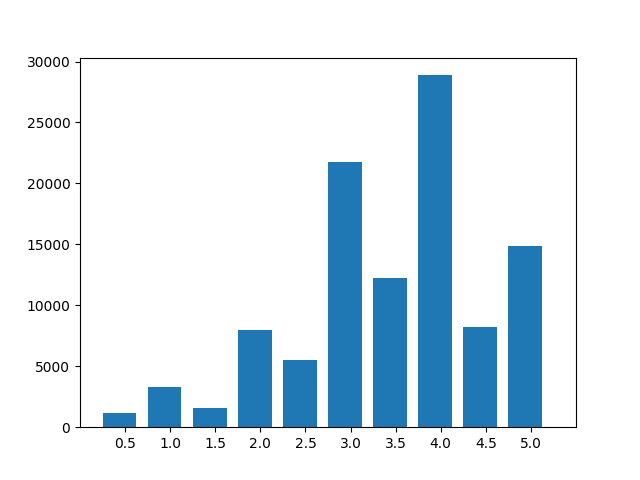
\includegraphics[scale=0.6]{small}
\caption{\emph{small} Movielens dataset ratings distribution}
\end{figure}

\begin{table}[H]
\centering
\begin{tabular}{l|r}
number of users N&  6040 \\ 
number of items M& 3706 \\
average rating & 3.58156 \\
standard deviation & 1.1171 \\
\end{tabular}
\caption{\emph{1M} Movielens dataset statistics}
\end{table}

\begin{figure}[H]
\centering
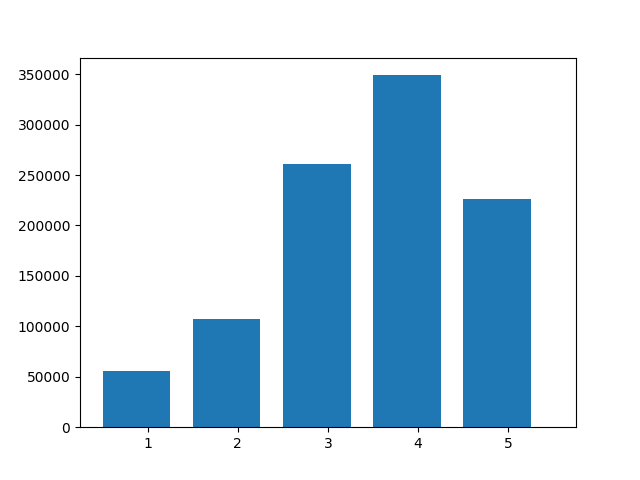
\includegraphics[scale=0.6]{1m}
\caption{\emph{1M} Movielens dataset ratings distribution}
\end{figure}


\section{Scaling issues and regularization}

In order to achieve the same intensity of learning per epoch even by varying
the minibatch size it is necessary to re-scale some hyperparameters.

Let's consider a complete objective for a typical learning task
of quantities $y_i$ from respective datapoints $x_i$, using
a dataset $\mathcal{D} = \{x_i,y_i\}_i^{|D|}$.
As the datapoints
are independent and identically-distributed, then it can be expressed as a sum over
all the datapoints.
One step of learning from this objective is usually referred as an "epoch".

\begin{nalign}
\label{complete_J}
J = \sum_{i=1}^{|\mathcal{D}|}
\ell(x_i,y_i) + \lambda \Omega(\Theta)
\end{nalign}

Where $\Omega$ is a regularization term, $\Theta$ is the set of the regularizable
parameters and $\lambda$ is a fixed hyperparamter that determines the regularization amount.

This objective is subject to Gradient Descent learning on the trainable parameters:

\begin{nalign}
\Theta_{t+1} = \Theta_t - \gamma\nabla_\Theta J_t
\end{nalign}

Where $\gamma$ is the learning rate hyperparameter.

As $J$ is defined as a sum over independent datapoints, it is possible to use Stochastic
Gradient Descent learning strategies, which take into account only a limited number of datapoints at each time.

It's desirable to consider the average contribution of each datapoint to the objective
$J$ \ref{complete_J}:

\begin{nalign}
\label{average_datapoint_J}
J_a = 
\frac{1}{|\mathcal{D}|}
J =
\frac{1}{|\mathcal{D}|}
\sum_{i=1}^{|\mathcal{D}|}
\ell(x_i,y_i) + \frac{\lambda}{|\mathcal{D}|} \Omega(\Theta)
\end{nalign}

If learning using $J_a$ is repeated $|\mathcal{D}|$ times within an epoch, then
the algorithm achieves the same learning intensity as
with $J$ by keeping the same learning rate $\gamma$.

By considering splitting the dataset and the objective $J$ 
\ref{complete_J} into a number of minibatches of size $B$, an approximation to $J_a$,
useful for SGD-like algorithms,
can be obtained:

\begin{nalign}
J_b = \frac{1}{B}\sum_{i=1}^{B} \ell (x_i, y_i) + \frac{\lambda}{|\mathcal{D}|}\Omega(\Theta)
\end{nalign}

An important consequence of using $J_b$ is that the intensity of the learning 
is altered,
because less updates would be applied to $\Theta$ at each epoch.
In order to balance this phenomenon, the learning rule can be modified as follows:

\begin{nalign}
\Theta_{t+1} = \Theta_t - B\gamma\nabla_\Theta J_{b,t}
\end{nalign}



\section{Prevention of exploding gradients}
It is possible, under specific circumstances, that the gradients may become unstable and
compromise the parameters of the model with infinities or "not a number" values.

In order to prevent this phenomenon, a few "tricks" have been implemented:

\paragraph{Gradient clipping}\cite{norm_clip} has been implemented with the
following norm-based scaling algorithm:

\begin{algorithm}
\caption{Norm-based gradient clipping}
\begin{algorithmic}[1]

\REQUIRE ~~\\
(1) Gradient tensor $\mathbf{g}$   \\
(2) Threshold $\theta$ (defaulted to value 10)
\ENSURE~~\\
(1) Scaled gradients $\hat{\mathbf{g}}$ whenever their L2 norm surpasses a threshold $\theta$.
`
\item[]
\IF{$||\mathbf{g}||_2 > \theta$}
    \STATE $\hat{\mathbf{g}} \leftarrow \frac{\theta}{||\mathbf{g}||_2}\mathbf{g}$
\ELSE
    \STATE $\hat{\mathbf{g}} \leftarrow \mathbf{g}$
\ENDIF
\RETURN $\hat{\mathbf{g}}$
\end{algorithmic}
\end{algorithm}

\paragraph{Scaled $\tanh$ activation function}. Some layers have 
"$\log\sigma$" outputs. As the output of these layers needs to be processed to
exponentiation in the likelihood function, if the activation is kept linear
there is a great risk of instability and value explosion.
For these reason a "pseudo-linear" soft-bounded activation function has been implemented
by re-scaling a $\tanh$ activation function.
A $\tanh$ activation function has the co-domain of the function bounded between -1 and +1.
Moreover, its derivative is approximately $1$ near the origin. It follows that $\tanh$
perfectly suits the role of pseudo-linear bounded activation function if it's rescaled as
follows:

\begin{nalign}
f(\mathbf{x}) = K * \tanh(\mathbf{x}/K)
\end{nalign}

Where $K$ is a small integer which is greater than 1. In this way this activation function
will be bounded between $-K$ and $+K$. A good value for $K$ might be 5, in order to obtain
$\sigma$-values properly bounded between $0.0067$ and $148.4$.

For layers that are supposedly linear in their outputs, such as Planar Flow's 
$\mathbf{w}$, $b$, and $\mathbf{u}$ quantities, as well as the means $\boldsymbol\mu$ of 
the gaussian distributions,
a "pseudo-linear" function
on the same guise has been implemented with $K=20$. 

\paragraph{Learning rate "warm-up"} has been implemented to prevent immediate divergence
in the first epochs due to steep gradients. 
Hence, the learning rate has been raised from a very small value
to regimen value during the course of the very first epochs.

\begin{algorithm}
\caption{Learning rate warm-up}
\begin{algorithmic}[1]

\REQUIRE ~~\\
(1) Initial learning rate $\gamma$   \\
(2) Current epoch number $t$ \\
(3) Number of initial warm-up epochs $K$ \\
(4) Base value of the warm up coefficient $B$  which has to be less than $1$
\ENSURE~~\\
(1) Adjusted and progressively increasing learning rate $\hat{\gamma}$ during the first $K$ epochs
\item[]
\IF{$t >= K$}
    \STATE $\hat{\gamma} = \gamma$
\ELSE
    \STATE $\hat{\gamma} = B^{K-t} \gamma$
\ENDIF
\RETURN $\hat{\gamma}$
\end{algorithmic}
\end{algorithm}

Appropriate parameter settings have been found as $K=3$ and $B=0.1$.


\section{Soft Free Bits settings}

During experiments with VaeRec, it was noted how the $\justkl$ values differ greatly from
the marginals to the $\justkl$.
This is because as the latent dimensionality increases, it gets harder to match
the prior and the posterior.
For this reason, for larger latent dimensionalities,
it can be observed a posterior collapse trough the $\justkl$ marginals,
even if the $\justkl$ still returns values that are reasonably high.

Within our \emph{Soft Free Bits} (see section \ref{posterior_collapse}) implementation
our solution was just to set the $\lambda$ linearly proportional to $K$, as in $\lambda=2*K$.

The annealing $\epsilon$ was set, as suggested in \cite{1611.02731}, to the value $0.05$.
The value of $\gamma$ was updated at every minibatch learning iteration.

\begin{figure}[H]
\centering
\includegraphics[scale=0.5]{kl_annealing1.png}
\caption{Free Soft Bits: evolution of kl annealing coefficient vs. kl divergence. The values are sampled after evey minibatch update. This plot has been obtained with about 50 epochs of VaeRec, without Normalizing Flows and with latent dimensionality K=1. In blue: annealing coefficient value; in green: KL measure}
\label{kl_annealing1}
\end{figure}


\begin{figure}[H]
\centering
\includegraphics[scale=0.5]{kl_annealing2.png}
\caption{Zoom-in of the last part of the previous figure \ref{kl_annealing1} . It is noticeable how the KL divergence measure succesfully converges towards the desired amount of 2. The annealing coefficient keeps oscillating, reflecting the dynamic nature of the annealing-vs-kl system. In blue: annealing coefficient value; in green: KL measure}
\label{kl_annealing2}
\end{figure}

\begin{figure}[H]
\centering
\includegraphics[scale=0.5]{kl_annealing_K=5_1bis.png}
\caption{Similar plot to \ref{kl_annealing1}, but with the more interesting case of K=5. The KL divergence also succesfully converge to the target value 10. In blue: annealing coefficient value; in green: KL measure}
\label{kl_annealing_K5_1}
\end{figure}

\begin{figure}[H]
\centering
\includegraphics[scale=0.5]{kl_annealing_K=5_2bis.png}
\caption{Zoom-in of the last part of the previous figure \ref{kl_annealing_K5_1}.  The annealing coefficient converges, with oscillations, towards small values such as the case with K=1.  In blue: annealing coefficient value; in green: KL measure}
\label{kl_annealing2}
\end{figure}


\section{Choice of hyperparameters}

The search for an acceptable model via hyperparameter search was a very long process.
Since most experiments took about 8 days to complete, choosing the right hyperparameter
settings took many months.

At the end of this process it was understood that most hyperparameters were located
on a specific trade-off minimum in a convex curve of validation error.
For example, using minibatch of size 1 gave
often unsatisfactory resuls. Better results were obtained with a minibatch of size 64,
but increasing that value, for example to 128 or 256 gave worse results.

Other hyperparameters that were problematic to set were those dedicated to 
L2 regularization of the network weights. A good balance was found by using 100 or 200 
as L2 regularization coefficient.

The learning rate was also located as a minimum in a convex curve.
High learning rates might initially progress faster but may "jump over" good minima,
while lower learning rates might converge to a better minima but take a larger amount of
epochs. These effects might be mitigated by the use of moment-based descent algorithm,
such as
Adam \cite{KingmaB14} and by the use of 
the learning rate annealing described in section \cite{annealing}, with
parameter $T$ set at $10$, meaning that the initial halving of the learning rate
happens after the first $10$ epochs (further decay is much slower)
. A good initial learning rate was found being 2e-6.

The ideal number of epochs would have been $1000$ but unfortunately reaching
this target was highly inpractical by the sheer amount of time that the training
required. This fact was aggravated by the limit on the number of concurrent
jobs that was imposed by the distributed supercomputer DAS4 administration,
which was about 10-20 long-running jobs at the same time.
For these reasons many reported experiments have been trained for a lower number of
epochs.

The depth of the network was finally chosen to be 1 hidden layer,
as it eases the creation of useful intermediate-level
representation values, as opposed to not using hidden layers at all. Latent dimensionalities explored were 5, 250 and 500. 




\section{Normalizing Flows}

Experiments with planar and RealNVP normalizing flows have been performed.
A base VaeRec model has been chosen with 1 hidden layer with dimensionality 1000, latent dimensionality 5, learning rate annealing T=10, and soft free bits' $\lambda=2*K=10$.

To this base model Normalizing Flows have been applied with 1 or 5 transformation steps.

\begin{figure}[H]
\centering
\includegraphics[scale=0.6]{realnvp_nf.png}
\caption{VaeRec with RealNVP Normalizing flows}
% python3 plot_3.py  harvest_vaerec_20180805_172533 harvest_vaerec_20180805_175835 harvest_vaerec_20180807_090728 '0 steps'  '1 step' '5 steps' --save text/realnvp_nf.png
\label{realnvp_nf_fig}
\end{figure}


\section{Equivalences between AutoRec and VaeRec models}

In order to perform an adequate comparison between the AutoRec and VaeRec
models it's important to establish if there are any available equivalences.
In other words, it is interesting to see if a specific choice of hyperparameters
of the VaeRec leads to a model that is similar to the VaeRec both in its definition
and its performance.

Luckily such a model can be found in the VaeRec by setting the KL coefficient to 0.
This way that extra regularization term is absent and the VaeRec model becomes analogous
to the AutoRec model. An hypothesis can be formulated that in such similar models
the performances will be similar as well.

Experimental results confirm the hypothesis:

\begin{table}[H]
\centering
\begin{tabular}{c|c|c|c|r|r}
\thead{Minibatch \\size }& 
\thead{hid.layer \\ width }& 
\thead{num. hidden \\layers } &
\thead{latent z \\ dimensionality} & 
\thead{AutoRec (RProp) \\ testing RMSE }&
\thead{VaeRec (Adam) \\ testing RMSE }
\\
\hline
64 & 1000 & 1 & 250 & 
% harvest_autorec_20180625_122221 (adam)
0.8700
% harvest_autorec_20180723_114300 (pseudo_linear, and adam)
WAITING
& 
% harvest_vaerec_20180608_231009
0.8335
% harvest_vaerec_20180723_110214 (pseudo_linear)
WAITING
\\
64 & 1000 & 2 & 250 & 
% harvest_autorec_20180427_022040
0.8341 
% harvest_autorec_20180723_120629 (pseudo_linear, and adam)
WAITING
% harvest_autorec_20180723_122618/ (adam)
WAITING
& 
% harvest_vaerec_20180608_224259
0.8365 
% harvest_vaerec_20180723_115919 (pseudo_linear)
WAITING
\\
64 & 1000 & 1 & 500 & 
% NO (rprop)
% NO (adam)
% harvest_autorec_20180725_005108/ (pseudo_linear, and adam)
WAITING
& 
% NO (no gradient hacks)
% harvest_vaerec_20180725_004522/ (pseudo_linear)
WAITING
\\
64 & 1000 & 2 & 500 & 
% NO (rprop)
% NO (adam)
% harvest_autorec_20180725_005647/ (pseudo_linear, and adam)
WAITING
& 
% NO (no gradient hacks)
% harvest_vaerec_20180725_010335/ (pseudo_linear)
WAITING
\end{tabular}
\caption{Comparison of similar VaeRec and AutoRec models}
\end{table}

The testing error achieved by both AutoRec and VaeRec models
are very similar under similar hyperparameter settings.

\section{User+Item concatenation vs traditional Item or User datapoints }
\subsection{User+Item concatenation on AutoRec}

For this experiment the base model AutoRec was used, with the purpose to
observe difference in learning outcomes between using just item vectors
versus the concatenation of user and item vectors.

For this experiment, a latent dimensionality of 250 and
with hidden layer dimensionality set at 500. These hyperparameters
reflect typical settings from the original AutoRec paper \cite{Sedhain2015}.
L2 regularization was set at 200.

\begin{figure}[H]
\centering
\includegraphics[scale=0.6]{autorec_ui.png}
\caption{AutoRec: comparing item learning vs user+item learning}
% python3 plot_2.py harvest_autorec_20180102_181908 harvest_autorec_20180104_111755 'item' 'user+item' --maxerr 3 --minerr 0 --epochs 800 --save text/autorec_ui.png
\label{autorec_ui_fig}
\end{figure}

Unfortunately the user+item version is not able to generalize well on the dataset,
Nevertheless it's interesting to see how the user+item version overfits more than 
the item version.
This indicates that using user+item concatenation datapoints might lead to better
performance on the test set if a suitable regularization method is found.

One disadvantage of using user+item was the much longer times for training, likely
because of the datapoint dimensionality increase.

\subsection{User+Item concatenation on VaeRec}

Similar comparison experiments have been performed on VaeRec,
with different model hyperparameters.
Specifically, these experiments differ by having used a much lower dimensionality
(5), which might have regularizing effects, as well as L2 regularization set at 100
and hidden layer dimensionality set at 1000. Moreover, learning rate annealing $T$
parameter has been
set to 10 and \emph{soft free bits} have been employed with $\lambda=2*K=10$.

\begin{figure}[H]
\centering
\includegraphics[scale=0.6]{vaerec_ui.png}
\caption{VaeRec: comparing item learning vs user+item and user learning}
% python3 plot_4.py harvest_vaerec_20180805_172533  harvest_vaerec_20180805_173309 harvest_vaerec_20180805_171337 harvest_vaerec_20180804_173844 'item lambda=10'  'user lambda=10' 'user+item lambda=10' 'user+item lambda=1' --epochs 120 --save text/vaerec_ui.png --maxerr 2 --minerr 0.75
\label{vaerec_ui_fig}
\end{figure}

Similarly as the previous AutoRec experiment, it can be observed how user+item overfits and performs poorly on the testing
set.

Interestingly, the 'user' version of VaeRec performs better than the baseline 'user' variant
of AutoRec as reported in their paper.

\begin{table}[H]
\centering
\caption{VaeRec: performance on the test set of item learning vs user+item and user learning, compared to the reported AutoRec outcomes \cite{Sedhain2015}}
 \begin{tabular}{||l | c c |c||} 
 \hline
 & \multicolumn{2}{c}{VaeRec} & AutoRec \\ \hline
 & training & testing & testing \\ \hline
item $\lambda=10$& 0.8240&0.8599 & 0.831 \\
user $\lambda=10$ & 0.8262&0.8598 & 0.874 \\
user+item $\lambda=10$ & 0.8241 & 1.0893 & N/A\\
user+item $\lambda=1$ &0.9813 & 0.9930 &\\
\hline
\end{tabular}
\end{table}

In these experiments using $\lambda=1$ very soon leads to NaN (Not A Number) 
interruption. This lead to the observation that there exists a lower-bound to the
$\justkl$ divergence, in this case about 2.46, which causes the annealing coefficient
to diverge towards infinity.

\section{Experiments with regularization techniques}

\subsection{Dropout layer on the input}

Denosing autoencoders\cite{denoising} improve the quality of the representations
by forcing resiliance of the neural network by adding noise on the input
and using the original datapoint in the objective function.

We tried a similar mechanism on our AutoRec re-implementation
by adding a Dropout \cite{Srivastava2014} layer with parameter $p=0.1$ on the input. 

The following plot shows that an improvement in generalization is indeed obtained:


\begin{figure}[H]
\centering
\includegraphics[scale=0.6]{autorec_input_dropout.png}
\caption{Dropout layer on the input of an AutoRec model}
% python3 plot_2.py  harvest_autorec_20180108_154116 harvest_autorec_20180120_124230 'without input dropout'  'input dropout p=0.1' --save text/autorec_input_dropout.png --epochs 627 --minerr 0.7 --maxerr 1.0
\label{input_dropout_fig}
\end{figure}

\subsection{Tradeoff between KL divergence and weights regularization}

Both weights decay and KL divergence are regularizers that enable the model to achieve
generalization. The contribution of both these terms is compounded, so that 
coefficients need to be tuned in order to avoid over-regularization.

As an example, this can be seen in the following plot, where a VaeRec model
using L2 regularization with coefficient 200 is tested with, and without
the KL term:

% python3 plot_2.py harvest_vaerec_20180602_151546 harvest_vaerec_20180530_220845 "with kl" "without kl" --save text/with_kl_vs_without_kl.png
\begin{figure}[H]
\includegraphics[scale=0.7]{with_kl_vs_without_kl.png}
\caption{VaeRec with and without KL divergence, minibatch size set at 1}
\end{figure}

For additional comparison, here are the result by using a minibatch update schema
with size set at 64:

\begin{figure}[H]
\includegraphics[scale=0.7]{with_kl_vs_without_kl_mb64.png}
\caption{VaeRec with and without KL divergence, minibatch size set at 64}
\end{figure}

Using the minibatch shows considerable improvements for both variants (with and without KL
divergence).  It is interesting how the model with KL improves in such a drastic way
by using minibatch learning. This is probably caused by the KL regularizer being
very noisy with individual samples, causing over-regularization, as typical with SGD
(without minibatch) schemas. By using a minibatch
the KL regularizer becomes less noisy by smoothening via averaging. 

